% IEEE Conference paper: Mixed-Precision Attention on Consumer Blackwell.
% Build: `make` (latexmk -pdf), or
%   pdflatex main && bibtex main && pdflatex main && pdflatex main
\documentclass[conference]{IEEEtran}
\IEEEoverridecommandlockouts

% --- packages -----------------------------------------------------------------
\usepackage[utf8]{inputenc}
\usepackage[T1]{fontenc}
\usepackage{microtype}
\usepackage{cite}
\usepackage{amsmath,amssymb,amsfonts}
\usepackage{algorithmic}
\usepackage{graphicx}
\usepackage{textcomp}
\usepackage{xcolor}
\usepackage{booktabs}
\usepackage{multirow}
\usepackage{siunitx}
\usepackage{listings}
\usepackage[hidelinks]{hyperref}
\usepackage{url}
\usepackage{array}

\sisetup{
  detect-all,
  group-separator={,},
  table-number-alignment=center,
  round-mode=places,
  round-precision=2,
}

\lstset{
  basicstyle=\ttfamily\footnotesize,
  breaklines=true,
  columns=fullflexible,
  keepspaces=true,
  showstringspaces=false,
  frame=none,
}

% --- title block --------------------------------------------------------------
\title{Mixed-Precision Attention on Consumer Blackwell:\\
A Pareto Replication Study from FP32 to NVFP4 on the RTX~5080}

\author{
  \IEEEauthorblockN{Anonymous Author(s)}
  \IEEEauthorblockA{Affiliation withheld for review}
}

% --- document -----------------------------------------------------------------
\begin{document}
\maketitle

\begin{abstract}
We replicate a decade of attention-kernel optimizations on the NVIDIA
RTX~5080, a mid-tier consumer Blackwell GPU underrepresented in
published kernel-level work. Five hand-rolled kernels share a common
algorithmic skeleton---tile streaming with online softmax---and differ
only in numerical precision and one optimization at a time, so each
step in the ladder isolates exactly one variable. We report three
findings. First, fusing the kernel and adopting online softmax cuts
peak HBM at sequence length 8192 by $17\times$, exactly matching
PyTorch's SDPA baseline, with no precision change. Second, a hand-rolled
FP8 kernel using \texttt{mma.sync m16n8k32} closes about half of the
remaining latency gap to SDPA, exploiting a hardware lever the vendor
library does not engage on this software stack. Third---and contrary to
the prevailing assumption that lower precision always wins---NVFP4 with
software microscaling is roughly $30\%$ \emph{slower} than FP8: the
per-mma scaling cost dominates the FP4 throughput advantage. The
hardware-microscaled NVFP4 path would plausibly invert this result, but
its scattered-fragment layout is incompatible with the row-major SMEM
idiom shared by our other variants, and we treat it as deferred work.
The full benchmark, kernels, and figure regeneration are reproducible
on a single 16~GB consumer GPU.
\end{abstract}

\begin{IEEEkeywords}
attention, mixed precision, FP8, NVFP4, FlashAttention, GPU kernels,
Tensor Cores, consumer Blackwell, sm\_120a, reproducibility
\end{IEEEkeywords}

% =============================================================================
\section{Introduction}
\label{sec:intro}

Attention is the dominant cost in modern transformer inference, both in
compute and in memory. Its quadratic dependence on sequence length has
driven a decade of kernel-level optimizations: tiling, fusion, online
softmax, and progressively narrower numerical formats. On datacenter
GPUs (H100, B100, B200), each of these ideas has been validated
independently, often more than once. On the flagship consumer card
(RTX~5090), recent work confirms that the optimizations transfer.

The mid-tier consumer card---the RTX~5080---has received much less
attention. It shares a compute capability (sm\_120a) with the 5090 but
differs on every other dimension that matters for kernel design: half
the SM count, a narrower memory bus, and a tighter VRAM ceiling. As a
practical inference target for individual researchers, small labs, and
edge deployments, it is arguably the more important platform. As an
object of academic study, it is essentially absent from the literature.

\subsection*{What this paper does}

We perform a controlled, ladder-style replication of mixed-precision
attention on the RTX~5080. We hand-roll five attention kernels that
share one algorithmic skeleton---tile streaming with online softmax,
single-kernel fusion, and (from the third kernel onward) a register-
resident output accumulator---and that differ only in numerical
precision and one specific optimization at a time. The kernels are:

\begin{itemize}
  \item \textbf{V0 (FP32, naive).} Three separate kernel launches with
        the full $N\times N$ score and probability matrices materialized
        in HBM. Serves as the \emph{correctness oracle} and as the
        worst-case latency/memory baseline.
  \item \textbf{V1 (FP16, tiled).} Same three-launch structure as V0,
        but with FP16 inputs and Tensor-Core matmuls via the
        \texttt{nvcuda::wmma} API. Isolates the contribution of
        \emph{tiling and Tensor-Core engagement} alone.
  \item \textbf{V2 (FP16, fused).} Single fused kernel with the online
        softmax recurrence; no longer materializes the score or
        probability matrices in HBM. Isolates \emph{algorithmic
        fusion}.
  \item \textbf{V3 (FP8, fused).} Hand-rolled FP8 (E4M3) kernel using
        inline-PTX \texttt{mma.sync.m16n8k32}, with a register-resident
        output accumulator and per-tile FP8 scaling. Isolates
        \emph{narrower-precision Tensor Cores}.
  \item \textbf{V4 (NVFP4, fused).} Same structure as V3, with the FP8
        mma replaced by the FP4 (E2M1) sync mma and software-managed,
        per-row, per-K-block microscaling. Isolates \emph{FP4
        precision}.
\end{itemize}

This ladder is constructed so that each step changes exactly one design
choice. The performance and accuracy delta at each step therefore
quantifies the contribution of that one choice on this hardware, with
no confounding.

\subsection*{Three findings}

Of the four steps in the ladder, two confirm the published trajectory,
one reveals an underappreciated software-stack confound, and one is a
clean negative result.

\textbf{The memory wall breaks at V2.} Adding online softmax and fusion
reduces peak HBM at sequence length 8192 from 2,176~MB to 128~MB---a
$17\times$ reduction that exactly matches the SDPA baseline---without
any precision change. The full $N\times N$ probability matrix is the
problem; once it stops being materialized, the memory footprint
collapses to the input/output footprint, and a 16~GB consumer card
becomes capable of sequence lengths it could not previously fit.

\textbf{V3 closes about half the SDPA gap with FP8.} V3 is $2.4\times$
faster than V2 and reaches roughly half of SDPA's throughput. This is
not because V3 has a better algorithm than the vendor library; it does
not. It is because the SDPA implementation that ships with PyTorch on
this stack \emph{does not} engage FP8 Tensor Cores at all---it
dispatches to a pair of cuBLAS matmuls with a softmax in between
(Section~\ref{sec:exp}). A custom kernel that uses a precision the
vendor library does not engage exposes a real hardware lever, even
when the algorithm is otherwise unchanged.

\textbf{V4 loses to V3 by $\approx 30\%$.} On the consumer-Blackwell
software stack we target, the per-mma overhead of software microscaling
exceeds the FP4 throughput advantage. This is the first quantitative
evidence we are aware of that low-precision attention is not strictly
Pareto-dominant on consumer Blackwell, in contrast to the purely
positive findings reported on H100 and RTX~5090. The hardware-
microscaled NVFP4 instruction family would likely invert the result,
but engaging it requires a different shared-memory layout we share
between V3 and V4, and we document this as deferred work.

\subsection*{Contributions versus prior work}

We do not introduce a new attention algorithm. The algorithmic
skeleton (online softmax, single-kernel fusion) is from
FlashAttention~\cite{dao2022flashattention}; the FP8 forward-pass
recipe is from Micikevicius et al.~\cite{micikevicius2022fp8}; the FP4
microscaling format is the OCP/NVFP4 standard, demonstrated on RTX~5090
by SageAttention3~\cite{zhang2025sageattention3}. What we add is:

\begin{enumerate}
  \item \emph{A controlled five-point ablation} that isolates the
        contribution of each step in the optimization ladder on a
        single hardware/software stack. Existing FP4 attention
        papers~\cite{zhang2025sageattention3,zhang2026attnqat} present
        a single optimized kernel and compare against external
        baselines; the per-step contribution of fusion, FP8, and FP4
        is not separable from their results. Our ladder makes each
        step measurable.
  \item \emph{The first kernel-level mixed-precision attention study
        on the RTX~5080.} The RTX~5080 is included in
        SlideSparse~\cite{shao2026slidesparse} as a sparse-GEMM
        evaluation platform but not as an attention-kernel target;
        Knoop and Holtmann's broader consumer-Blackwell
        study~\cite{knoop2026consumerllm} explicitly omits the 5080
        in favor of the 5060~Ti, 5070~Ti, and 5090. Our V4 differs
        from SageAttention3 in three concrete ways
        (Section~\ref{sec:related}): SKU, mma instruction family, and
        ablation framing.
  \item \emph{A negative result on FP4 microscaling overhead.}
        SageAttention3 reports FP4 wins on RTX~5090 using the
        hardware-microscaled \texttt{mxf4nvf4} mma; we measure that
        when the same precision is forced through the
        software-microscaled \texttt{kind::f8f6f4} path---which is
        the only path compatible with row-major SMEM access---the
        per-mma overhead reverses the win. To our knowledge this is
        the first quantitative evidence that FP4 attention is not
        strictly faster than FP8 attention on consumer Blackwell, and
        it complements the failure-mode literature~%
        \cite{zhang2026attnqat,qiu2025lowprecisionfails,zhang2026snapmla}
        that documents why FP4 attention is hard.
  \item \emph{A backend-dispatch finding with methodological
        consequences.} On the PyTorch~2.9.1+cu128 Windows wheel we
        test, SDPA falls through to the \texttt{MATH} backend for
        sm\_120 / FP16 / non-causal inputs---attempts to pin
        \texttt{FLASH\_ATTENTION} or \texttt{CUDNN\_ATTENTION} are
        rejected at runtime. The performance baseline an end user sees
        is therefore not FlashAttention-2 on this stack. Existing
        attention papers comparing against ``SDPA'' without naming the
        dispatch are liable to mis-attribute speedups. We argue this
        is a community-wide methodology gap and recommend an explicit
        pinning convention.
\end{enumerate}

\subsection*{Roadmap}
Section~\ref{sec:bg} establishes necessary background.
Section~\ref{sec:related} positions our work against eight prior
contributions individually, with a comparison table.
Sections~\ref{sec:method}--\ref{sec:exp} describe the kernels and
methodology. Section~\ref{sec:results} presents results.
Sections~\ref{sec:disc}--\ref{sec:limits} discuss implications and
limitations, including a hardware-transfer table relating each of our
findings to its closest prior result.
Appendix~\ref{app:repro} is the reproducibility checklist.

% =============================================================================
\section{Background}
\label{sec:bg}

\paragraph*{Attention and its memory problem}
Standard scaled dot-product attention computes
\begin{equation}
\mathrm{Attn}(Q,K,V) = \mathrm{softmax}\!\left(\tfrac{1}{\sqrt{D}}\, Q K^\top\right) V,
\label{eq:attn}
\end{equation}
where $Q$, $K$, $V$ are $N \times D$ matrices of queries, keys, and
values, and the softmax is row-wise over the $N \times N$ score matrix
$S = QK^\top$~\cite{vaswani2017attention}. Materializing $S$ in
high-bandwidth memory (HBM) costs $O(N^2)$, which becomes the dominant
memory-traffic and latency bottleneck at long context.

\paragraph*{Online softmax}
FlashAttention~\cite{dao2022flashattention} eliminates the $S$
materialization by streaming over $K$ and $V$ in tiles and computing
partial softmax results tile-by-tile. The key trick is the
\emph{online softmax} recurrence: as each new tile arrives, the kernel
maintains a running per-row maximum and a running denominator, and
rescales the partial output to account for the new maximum. The
mathematical detail is in the original paper. For our purposes, two
properties matter: the recurrence is exact (it produces the same
numerical answer as the materialized version, up to floating-point
roundoff), and it has two boundary cases not stated in the
FlashAttention algorithm box but required for correctness---the first
iteration (running max is $-\infty$) and the fully-masked case
(causal padding past the diagonal), both of which can produce NaN if
not guarded explicitly. Our V2 kernel handles both. We adopt the
online-softmax structure in V2 through V4.

\paragraph*{Tensor Cores on consumer Blackwell}
5\textsuperscript{th}-generation Tensor Cores expose a family of
synchronous matrix-multiply-accumulate (\texttt{mma.sync})
instructions that consume operands of various widths and produce a
higher-precision accumulator. Three matter for this paper: the FP16
mma at width $16{\times}8{\times}16$ (V1, V2, via the high-level
\texttt{wmma} API); the FP8 (E4M3) mma at width $16{\times}8{\times}32$
(V3, via inline PTX); and the FP4 (E2M1) mma at width
$16{\times}8{\times}32$ (V4). The FP4 instruction requires the
architecture-accelerated \texttt{sm\_120a} target;
\texttt{ptxas} rejects it on the unsuffixed \texttt{sm\_120}, a
detail that ships with the V4 source tree but is otherwise easy to
miss. Each instruction places its operands in a per-thread register
fragment whose layout is fully specified in the PTX
ISA~\cite{nvidia2024ptxisa}. For the FP16 mma the layout is
implementation-defined, which has consequences for V2 we discuss in
Section~\ref{sec:method}.

A fourth instruction family, \texttt{mxf4nvf4.m16n8k64}, internalizes
a per-16-element scale factor at the hardware level and would in
principle deliver a faster FP4 attention than V4. CUTLASS exposes it
via \texttt{cute::SM120\_16x8x64\_TN}~\cite{nvidia2024cutlass}, but
its operand layout uses scattered per-thread fragments that are
incompatible with the row-major shared-memory idiom V1--V3 use.
Engaging it would require a different shared-memory layout
(\texttt{ldmatrix}-style swizzled access) and a CUTLASS-mediated
load, which is multi-week scope; we treat it as future work.

\paragraph*{What FP8 and FP4 can represent}
FP8 (E4M3) provides roughly 16 representable positive values with a
maximum magnitude of 448; FP4 (E2M1) provides roughly 6 representable
positive values with a maximum of 6. Per-tile or per-block scaling is
therefore not optional for either format: an unscaled tile of
attention probabilities, which lie in $[0,1]$ but with contrast that
varies dramatically across realistic workloads, would lose most of
its small-magnitude entries to underflow. V3 uses a single scale per
tile of $P$. V4 uses one scale per row per 32-element block of K---
finer granularity, more faithful to FP4's narrower range. The
empirical accuracy envelope of each is in Section~\ref{sec:results}.

\paragraph*{PyTorch SDPA dispatch is not a fixed reference}
\texttt{torch.nn.functional.scaled\_dot\_product\_attention} (SDPA)
is the standard PyTorch API for attention. At runtime it dispatches
to one of four backends based on a combination of build flags and
runtime capability checks: \texttt{FLASH\_ATTENTION},
\texttt{CUDNN\_ATTENTION}, \texttt{EFFICIENT\_ATTENTION}, or
\texttt{MATH}~\cite{pytorch2024sdpa}. The choice depends on the
PyTorch wheel, the CUDA version, the GPU compute capability, the
input dtype, the head dimension, the mask, and other factors. The
pinning context manager
\texttt{torch.nn.attention.sdpa\_kernel(SDPBackend.NAME)} forces a
specific backend or fails if it is unavailable. We use it in our
experiments to avoid a confound that has bitten the SageAttention3
results~\cite{zhang2025sageattention3} as well as ours: which
\emph{specific} backend SDPA picks materially changes ``the'' SDPA
performance, and a paper that does not pin and disclose the dispatch
is not measuring what it thinks it is.

% =============================================================================
\section{Related Work and Comparison to Prior Art}
\label{sec:related}

We position our work against eight specific prior contributions, then
summarize the comparison in Table~\ref{tab:prior_work}. The aim is to
make explicit, for each related paper, what they did, what we do, and
where the difference lies. We organize the discussion by category:
attention kernel optimization, mixed-precision attention (positive
findings), mixed-precision attention (failure modes), consumer
Blackwell ecosystem maturity, and reproducibility methodology.

\subsection{Attention Kernel Optimization}

\paragraph*{FlashAttention~\cite{dao2022flashattention}}
\emph{What they did:} introduced IO-aware tile streaming with online
softmax, eliminating the $N{\times}N$ score-matrix materialization;
A100 / FP16. \emph{What we do:} our V2 is a faithful FP16
re-implementation of this algorithmic skeleton on consumer Blackwell,
serving as the platform-on-which-fusion-was-tested baseline rather
than a competitor. \emph{Difference:} we replicate the algorithmic
contribution on a hardware tier the original work did not target, and
we do so as one rung of a controlled ladder rather than a standalone
optimized kernel.

\paragraph*{FlashAttention-3~\cite{shah2024flashattention3}}
\emph{What they did:} added Hopper-specific warp-specialized
pipelining via the Tensor Memory Accelerator (TMA) and introduced
FP8 (E4M3) throughput; H100. \emph{What we do:} our V3 borrows the
register-resident accumulator idea but implements it via hand-rolled
inline PTX. \emph{Difference:} TMA is absent on consumer
Blackwell~\cite{nvidia2025blackwell}, so the warp-specialized
pipelining does not transfer. The CUTLASS reference example for
Blackwell FMHA (\texttt{77\_blackwell\_fmha}) is gated to
sm\_100a/sm\_103a as of v4.4.2~\cite{nvidia2024cutlass}, leaving the
inline-PTX path as the only realistic implementation route on
sm\_120a. Our finding is consistent with FA-3's FP8-vs-FP16 latency
ratio in spirit, but the absolute numbers are tier-specific.

\paragraph*{FlexAttention~\cite{dong2025flexattention}}
\emph{What they did:} compiler-driven programming model that compiles
user-defined attention masks via \texttt{torch.compile}, achieving
within $\sim$30\% of hand-tuned kernels with much less code; PyTorch.
\emph{What we do:} we hand-roll kernels in CUDA and inline PTX.
\emph{Difference:} different optimization targets. FlexAttention
trades raw performance for programmability, ours trades
programmability for hardware-specific performance and a controlled
ablation. The two are complementary; FlexAttention is an
\emph{alternative} a deployer would consider, not a competitor on
the Pareto curve.

\paragraph*{vLLM PagedAttention~\cite{kwon2023vllm} and
vAttention~\cite{prabhu2024vattention}}
\emph{What they did:} serving-system primitives for KV-cache memory
management, with vAttention specifically documenting PagedAttention
decode-time regressions versus FlashAttention-2.
\emph{What we do:} we target the kernel itself, not the serving
system. \emph{Difference:} kernel-level vs system-level. Our V3 could
be plugged into either system; the comparison is orthogonal. We cite
these to mark them as the practical alternatives a deployed
inference stack would consider, not to compete with them.

\subsection{Mixed-Precision Attention: Positive Findings}

\paragraph*{Micikevicius et al.~\cite{micikevicius2022fp8}}
\emph{What they did:} formalized E4M3 / E5M2 FP8 formats and
delayed-scaling recipe for mixed-precision training; H100.
\emph{What we do:} adopt the forward-pass E4M3 recipe in V3.
\emph{Difference:} we apply it to inference attention specifically,
not training; we use per-tile static scaling rather than delayed
scaling because forward-only inference does not require optimizer-
state preservation; we add the V3-vs-V4 comparison that they could
not (FP4 hardware did not exist).

\paragraph*{SageAttention~\cite{zhang2025sageattention} (the original 8-bit work)}
\emph{What they did:} demonstrated that 8-bit attention is
plug-and-play deployable; outperforms FlashAttention-2 by $\sim
2.1\times$ and xformers by $\sim 2.7\times$ on Hopper; ICLR 2025.
\emph{What we do:} V3 demonstrates the same trajectory on consumer
Blackwell. \emph{Difference:} hardware tier (Hopper vs sm\_120a),
SDPA-baseline backend (FlashAttention-2 vs MATH-backend cuBLAS), and
framing (standalone optimized kernel vs ladder ablation). Our V3's
$2.4\times$ over V2 is consistent with their $\sim 2.1\times$ over
FlashAttention-2 in spirit, but the absolute numbers are not
directly comparable because the baselines differ.

\paragraph*{SageAttention3~\cite{zhang2025sageattention3}}
This is our closest related work. We treat it in detail.

\emph{What they did:} demonstrated NVFP4 attention on RTX~5090
(Blackwell consumer flagship, sm\_120a) using the
hardware-microscaled \texttt{mxf4nvf4.m16n8k64} mma family with the
NVFP4-standard 16-element block; reported throughput exceeding
FlashAttention-3's FP8; NeurIPS 2025 Spotlight.

\emph{What we do:} V4 attempts the FP4 attention transfer to
RTX~5080 using the software-microscaled
\texttt{kind::f8f6f4.m16n8k32} path with a 32-element block, and
reports a negative result---V4 is $\approx 30\%$ slower than V3 (FP8)
on this hardware/software combination.

\emph{Difference, in three concrete dimensions:}
\begin{itemize}
  \item \emph{Target SKU.} RTX~5090 has 170 SMs, 32~GB GDDR7, and a
        512-bit memory interface. RTX~5080 has 84 SMs, 16~GB GDDR7,
        and a 256-bit interface. Both are sm\_120a, but the per-SM
        cache topology, register pressure budget, and HBM bandwidth
        differ enough that ``it works on 5090'' does not imply
        ``it works on 5080.''
  \item \emph{Instruction family.} SageAttention3 uses
        \texttt{mxf4nvf4.m16n8k64}, which internalizes per-16-element
        scaling at the mma boundary. We use
        \texttt{kind::f8f6f4.m16n8k32}, which requires software
        microscaling. The two paths are not interchangeable: the
        hardware path's scattered per-thread fragments are
        incompatible with the row-major SMEM idiom we share with V3.
        Engaging the hardware path would require a different SMEM
        layout (\texttt{ldmatrix}-style swizzled access) we estimate
        at multi-week scope.
  \item \emph{Framing.} SageAttention3 is a standalone optimized
        kernel; per-step contributions of fusion, FP8, and FP4 are
        not separable from their results because they only present
        the final FP4 number. Our ladder presents V0/V1/V2/V3/V4
        side by side, so the contribution of \emph{each} step on
        the same hardware is measurable. The negative V4 result
        therefore says something specific---``software microscaling
        overhead exceeds FP4 throughput advantage''---rather than
        ``FP4 does not work,'' which would be inconsistent with
        SageAttention3's positive result on hardware microscaling.
\end{itemize}

We do not aim to outperform SageAttention3; we cite their FP4
throughput as the upper bound the hardware-microscaled path would
deliver on a related platform.

\subsection{Mixed-Precision Attention: Failure Modes}

The following three works share with us the position that
low-precision attention is not always Pareto-dominant. We
contextualize each.

\paragraph*{Attn-QAT~\cite{zhang2026attnqat}}
\emph{What they did:} first systematic study of 4-bit
quantization-aware training for attention; identified that the
natural FP4 forward + high-precision FlashAttention backward recipe
is unstable and proposed two principles for stability (matching
low-precision recomputation and resolving FA's implicit precision
assumptions); RTX~5090, 1.5x diffusion-model speedup; preprint 2026.
\emph{What we do:} forward-pass inference only, no QAT; V4 reports
the per-mma cost of forward FP4 attention with software
microscaling. \emph{Difference:} our scope is forward inference;
theirs is training. The two are complementary failure-mode
characterizations: theirs explains why naive FP4 training diverges,
ours quantifies why naive FP4 inference does not always win on
consumer hardware. The bulk-correctness envelope we measure
(rel-L2 of $\approx 0.21$ at unit variance for V4) sits below the
threshold where Attn-QAT-style intervention would be necessary, but
our negative latency result says inference-time FP4 deployment
faces an additional hurdle they do not address.

\paragraph*{Qiu and Yao~\cite{qiu2025lowprecisionfails} (``Why Low-Precision Fails'')}
\emph{What they did:} mechanistic explanation of catastrophic loss
explosion in low-precision FlashAttention training; identifies the
joint effect of (a) emergence of similar low-rank representations
within attention and (b) compounding biased rounding errors in the
online softmax recurrence; proposes a minimal modification to flash
attention that mitigates the rounding bias; ICLR 2026 poster.
\emph{What we do:} we measure the inference-time consequence of the
same online-softmax-recurrence rounding pattern: V3's
contrast-dependent error envelope (Section~\ref{sec:results}) shows
a roughly linear growth in relative error with input variance,
consistent with the bias-accumulation mechanism Qiu and Yao
identify. \emph{Difference:} they target training stability and
weight updates; we target inference accuracy and a stable
deployment recommendation. Their proposed modification could in
principle reduce V3's contrast-dependent floor, but we have not
tested it; this is one of several orthogonal extensions a future
artifact could integrate.

\paragraph*{SnapMLA~\cite{zhang2026snapmla}}
\emph{What they did:} characterized FP8 attention sub-types (RoPE-
bearing components, MLA decode, KV-shared structure) requiring
per-component precision retention; co-designs algorithm and kernel
for DeepSeek MLA decoding; up to $1.91\times$ throughput; preprint
2026. \emph{What we do:} per-tile (V3) and per-row, per-K-block
(V4) uniform scaling without component-aware retention.
\emph{Difference:} different masking and architecture target
(MLA decode in their case, dense non-causal forward in ours).
Their finding---that not all attention sub-tensors should be
quantized at the same granularity---argues that V3's contrast-
dependent error floor could be reduced by component-aware scaling,
but at the cost of additional kernel complexity. We do not pursue
this in V3 and document it as a defensible follow-up.

\subsection{Consumer Blackwell Ecosystem Maturity}

\paragraph*{vLLM RTX~5080/5090 setup~\cite{vllm2025issue14452} and CUDA~13 regression~\cite{vllm2025issue29030}}
\emph{What they did:} document concrete RTX 5080/5090 deployment
hurdles---CUDA 12.8 + container required, FA-3 backend not
working with Blackwell, undefined symbols in vLLM 0.11.1 under
CUDA~13.0 (\texttt{cutlass\_moe\_mm\_sm100} not a superset of
sm\_120). \emph{What we do:} document the V4 build's parallel
hurdle---\texttt{kind::f8f6f4} requires \texttt{sm\_120a}, not
\texttt{sm\_120}, and the runtime SDPA attempts to pin
\texttt{FLASH\_ATTENTION} are rejected at runtime.
\emph{Difference:} they target inference-server deployment; we
target kernel development. Both are evidence that the consumer-
Blackwell software stack is genuinely immature and that papers
in this space need to disclose the exact build under test.

\paragraph*{vLLM FlashInfer FP8 accuracy regression~\cite{vllm2026issue35138}}
\emph{What they did:} document a Blackwell-specific FP8 attention
correctness divergence in FlashInfer; recommend backend switch to
Flash-Attn rather than precision change. \emph{What we do:}
report that the SDPA FP16 path on this PyTorch build also has
non-obvious dispatch (falls through to MATH backend).
\emph{Difference:} their finding is a specific bug; ours is a
build-time configuration finding. Both reinforce the
methodological argument that the ``vendor baseline'' is a moving
target on consumer Blackwell.

\paragraph*{vLLM RTX 5080 NVFP4 pre-flight memory rejection~\cite{vllm2025issue30707}}
\emph{What they did:} document a 14~GB NVFP4 model + 2~GB KV cache
that fits in 16~GB but is rejected by overly aggressive
pre-flight validation. \emph{What we do:} report V4 actually
running on the same 16~GB card with NVFP4 weights, demonstrating
that the validation rejection is not a fundamental hardware
constraint. \emph{Difference:} they document a deployment
constraint; we demonstrate the underlying capability is present.
This is corroborating evidence for our claim that consumer-
Blackwell software is the binding constraint, not the hardware.

\subsection{Reproducibility and Hardware-Transfer Methodology}

\paragraph*{Pineau et al.~\cite{pineau2021reproducibility} and Desai et al.~\cite{desai2025reproducibility}}
\emph{What they did:} establish the reproducibility taxonomy and
checklist for ML research (Pineau, NeurIPS 2019 program report);
formalize repeatability vs.\ dependent / independent reproducibility
vs.\ direct / conceptual replication (Desai). \emph{What we do:}
position our work as a \emph{conceptual replication under hardware
shift} (Desai's terminology), and follow the Pineau checklist for
artifact release. \emph{Difference:} not a methodological
contribution---we are an instance of the framework. We cite to make
the positioning explicit.

\paragraph*{Kalibera and Jones~\cite{kalibera2013rigorous} and van der Kouwe et al.~\cite{vanderkouwe2018benchmarkingcrimes}}
\emph{What they did:} steady-state benchmark methodology and
catalog of benchmarking errors. \emph{What we do:} use 100 warmup
+ 500 timed iterations, paired CUDA events, p50/p95/p99 reporting,
disclosed clock state, paired-backend SDPA comparison (where
possible). \emph{Difference:} we apply their methodology to a
GPU-kernel context they did not explicitly target (their examples
are JVMs and security defenses). The principles transfer; the
specific defenses (paired CUDA events vs.\ wall-clock,
\texttt{cuobjdump}-based instruction inspection vs.\ admin-gated
profiler) are GPU-specific.

\paragraph*{Adjacent consumer Blackwell work~\cite{shao2026slidesparse,knoop2026consumerllm}}
\emph{What they did:} SlideSparse evaluates on a wide consumer +
datacenter GPU portfolio including the RTX~5080, but for sparse
GEMM, not attention. Knoop and Holtmann benchmark RTX 5060 Ti,
5070 Ti, and 5090 for inference but explicitly omit the 5080.
\emph{What we do:} kernel-level attention on the RTX~5080
specifically. \emph{Difference:} workload (sparse GEMM /
inference-server vs attention kernel) and SKU coverage (5080
included, vs 5080 omitted). The combination---kernel-level
attention on the RTX~5080---is, to our knowledge, original to
this paper.

\subsection{Comparison Summary}

Table~\ref{tab:prior_work} consolidates the above. Each row marks,
for one prior work, the dimension on which we differ.

\begin{table*}[t]
  \centering
  \caption{Comparison to Prior Work. Each row marks where our paper
    differs from one prior contribution. ``$\bullet$'' = same;
    ``$\circ$'' = different.}
  \label{tab:prior_work}
  \footnotesize
  \begin{tabular}{lccccccc}
    \toprule
    \textbf{Prior work} & \textbf{Same algo} & \textbf{Same precision} &
    \textbf{Same SKU} & \textbf{Same instr.\ family} &
    \textbf{Same scope} & \textbf{Same baseline} & \textbf{Our delta} \\
    \midrule
    FlashAttention~\cite{dao2022flashattention}        & $\bullet$ & $\bullet$ (FP16) & $\circ$ (A100) & $\circ$ (legacy mma) & $\bullet$ infer. & $\circ$ & RTX~5080 replication \\
    FlashAttention-3~\cite{shah2024flashattention3}    & $\bullet$ & $\bullet$ (FP8) & $\circ$ (H100)  & $\circ$ (TMA path)   & $\bullet$ infer. & $\circ$ & no-TMA tier, hand PTX \\
    FlexAttention~\cite{dong2025flexattention}         & $\circ$   & $\circ$ (FP16)   & $\circ$         & $\circ$ (compiler)   & $\bullet$ infer. & $\bullet$ & raw kernel vs compile \\
    PagedAttention~\cite{kwon2023vllm}                 & $\bullet$ & $\bullet$       & $\circ$         & $\bullet$            & $\circ$ serving  & $\circ$ & kernel level only \\
    Micikevicius FP8~\cite{micikevicius2022fp8}        & $\circ$   & $\bullet$ (E4M3) & $\circ$ (H100) & $\bullet$ FP8 mma    & $\circ$ training & $\circ$ & inference, per-tile \\
    SageAttention~\cite{zhang2025sageattention}        & $\bullet$ & $\bullet$ (FP8)  & $\circ$ (Hopper) & $\bullet$ FP8 mma  & $\bullet$ infer. & $\circ$ FA-2 & MATH-backend SDPA \\
    SageAttention3~\cite{zhang2025sageattention3}      & $\bullet$ & $\bullet$ (FP4)  & $\circ$ (5090)   & $\circ$ HW microsc. & $\bullet$ infer. & $\circ$ & 5080, SW microsc., ladder \\
    Attn-QAT~\cite{zhang2026attnqat}                   & $\bullet$ & $\bullet$ (FP4)  & $\circ$ (5090)   & $\circ$ HW microsc. & $\circ$ training & $\circ$ & forward only, no QAT \\
    Qiu \& Yao~\cite{qiu2025lowprecisionfails}         & $\bullet$ & $\bullet$ (BF16) & $\circ$         & $\circ$              & $\circ$ training & $\circ$ & inference manifestation \\
    SnapMLA~\cite{zhang2026snapmla}                    & $\circ$ MLA & $\bullet$ (FP8) & $\circ$         & $\bullet$            & $\bullet$ infer. & $\circ$ & dense, no MLA \\
    SlideSparse~\cite{shao2026slidesparse}             & $\circ$ GEMM & $\circ$        & $\bullet$ 5080  & $\circ$ sparse       & $\bullet$ infer. & $\circ$ & attention, not GEMM \\
    Knoop \& Holtmann~\cite{knoop2026consumerllm}      & $\circ$ infer. & $\circ$ mixed & $\circ$ (no 5080) & $\circ$ system    & $\circ$ system  & $\circ$ & 5080, kernel level \\
    \bottomrule
  \end{tabular}
\end{table*}

% =============================================================================
\section{Methodology}
\label{sec:method}

We implement five attention-kernel variants, each isolating one
optimization or precision change against its predecessor. All kernels
take FP16 inputs $(Q, K, V)$ and produce an FP16 output $O$, allowing
identical correctness tests across the ladder via a relative-L2
comparison against an FP32 reference. Common infrastructure---tile
sizing macros, dynamic-shared-memory opt-in, correctness oracle, FLOP
accounting---lives in \texttt{kernels/common/}.

\subsection{V0: FP32 Naive (Correctness Oracle)}

V0 materializes the full $N \times N$ attention matrix in HBM via
three separate kernel launches: a tiled $QK^\top$ matmul, a row-wise
softmax, and a $PV$ matmul. All three operate in FP32. V0 is
intentionally not optimized; its job is to be obviously correct and
to serve as the reference against which V1 through V4 are measured.

One subtle point worth flagging: the row-wise softmax requires a
\texttt{\_\_syncthreads()} between its two reduction phases (max-
subtract and normalize). Without it we observed a nondeterministic
$\sim 6\%$ output mismatch on sufficiently large $N$, which took
several hours to diagnose. V0 uses \texttt{--use\_fast\_math};
the impact on FP32 accuracy was below $10^{-6}$ across the test grid.

\subsection{V1: FP16 Tiled, WMMA Tensor Cores}

V1 keeps V0's three-launch structure but switches inputs to FP16 and
uses Tensor Cores for both matmuls via the \texttt{nvcuda::wmma}
API. Two design choices are worth flagging.

First, the $QK^\top$ matmul does not require an explicit transpose
pass: the WMMA B fragment accepts a column-major operand, and loading
$K$ (row-major in HBM) as column-major produces $K^\top$ implicitly.
No data movement, no extra kernel.

Second, on Blackwell the static \texttt{\_\_shared\_\_} arrays and
dynamic \texttt{extern \_\_shared\_\_} together count against a 48~KB
default per-block cap. V1's per-tile budget at $D = 128$ is exactly
48~KB, with no headroom. We allocate a single dynamic SMEM region
and \texttt{reinterpret\_cast} sub-regions out of it; this is a
precondition for V2's larger tile allocations.

V1 still materializes the score matrix $S$ and the probability
matrix $P$ in HBM. The intermediate $S$ tensor is the dominant
memory-bandwidth cost at long sequence lengths and is what V2's
fusion eliminates.

\subsection{V2: FP16 Fused (Online Softmax)}

V2 collapses the three V1 launches into a single fused kernel and
applies the online softmax recurrence (Section~\ref{sec:bg}). Per
$(\mathrm{batch}, \mathrm{head})$ pair we launch one block per
$\mathrm{B}_R$-row tile of $O$; the block iterates internally over the
$N / \mathrm{B}_C$ key/value tiles, maintaining the running max and
denominator across iterations and dividing by the denominator at the
epilogue.

The shared-memory layout at $D = 128$ totals 96~KB---over twice the
default cap. The launch silently fails without
\texttt{cudaFuncSetAttribute(\dots, MaxDynamicSharedMemorySize,
bytes)}. The RTX~5080 sm\_120 supports up to $\sim$99~KB per block;
we cache the attribute call behind a \texttt{static bool} so it is
paid once per process.

V2's main remaining performance limitation is structural rather than
algorithmic. The online-softmax update requires multiplying every
element of the running output accumulator by a per-row scalar at
each iteration. WMMA accumulator fragments have implementation-
defined per-thread layouts, so applying a per-row scalar to a
fragment requires either knowing the layout or doing a
layout-agnostic round trip through shared memory. V2 takes the
layout-agnostic route: store the accumulator to SMEM, apply the
rescale, reload it into a fragment for the next mma. This SMEM
round trip is the dominant remaining latency cost in V2, and it is
exactly what V3's hand-rolled \texttt{mma.sync} avoids. We template
the kernel by $\mathrm{HEAD\_DIM} \in \{64, 128\}$ so the inner-D
fragment count is a compile-time constant.

\subsection{V3: FP8 Fused with Hand-Rolled \texttt{mma.sync}}
\label{sec:method:v3}

V3 swaps V2's FP16 \texttt{wmma} matmul for the FP8 (E4M3)
\texttt{mma.sync} at width $16{\times}8{\times}32$, called via inline
PTX. The key advantage is that the \texttt{mma.sync} per-thread
fragment layout is \emph{fully specified} in the PTX ISA, not
implementation-defined as in WMMA. V3 keeps the output accumulator
in registers across the K/V iteration loop, replacing V2's SMEM
round trip with a per-iteration register-resident scaling.

\paragraph*{Why inline PTX rather than CUTLASS}
The natural CUTLASS reference for this kernel is
\texttt{77\_blackwell\_fmha}, but as of v4.4.2 it gates compilation
to sm\_100a/sm\_103a (the datacenter Blackwell parts that have
TMA). sm\_120a has no FMHA reference example, only GEMM
examples~\cite{nvidia2024cutlass}. Composing a V3-equivalent fused
multi-head attention from CUTLASS's \texttt{CollectiveBuilder}
primitives on sm\_120a would require manually composing the
warp-specialized persistent dispatch with a softmax-fused inner
loop---multi-week scope, and out of proportion to V3's marginal
complexity over V2. We use inline PTX following the
\texttt{cute::SM89\_16x8x32\_F32E4M3E4M3F32\_TN} register-layout
convention but do not link CUTLASS at build time.

\paragraph*{Per-tile FP8 scaling}
Each $Q$, $K$, and $V$ tile is rescaled cooperatively before being
quantized to FP8 and stored to SMEM. Each thread holds its slice of
the FP16 input in registers, contributes to a block-wide
\texttt{absmax} reduction, the published scale is broadcast back,
and the FP8 store proceeds register-to-SMEM with no FP16 staging
buffer. This halves the per-tile SMEM footprint relative to a
stage-then-quantize design. The probability matrix $P$ is rescaled
per-tile by a single scale derived from the tile-wide max of $P$.
This contrast-dependent FP8 scale is the dominant accuracy lever
for V3 and sets its empirical error envelope
(Section~\ref{sec:results}).

\paragraph*{$V$ stored col-major in SMEM}
The $16{\times}8{\times}32$ \texttt{mma.sync} requires the B operand
in column-major layout. We fold the transpose into the cooperative
load: each thread reads $V$ row-major from HBM and writes it
column-major to SMEM. Single pass, no extra kernel.

V3 emits 96 \texttt{QMMA.16832.F32.E4M3.E4M3} instructions in cubin
across the two HEAD\_DIM template instantiations, verifiable via
\texttt{cuobjdump --dump-sass | Select-String QMMA}. We use this
post-build check rather than Nsight Compute's runtime
Tensor-Core-engagement metric, which on consumer Blackwell is gated
behind admin-only \texttt{ERR\_NVGPUCTRPERM} permissions.

\subsection{V4: NVFP4 with Software Microscaling}
\label{sec:method:v4}

V4 extends V3's structure to NVFP4 (E2M1) using the software-
microscaled \texttt{mma.sync.aligned.kind::f8f6f4.m16n8k32.\dots\
.e2m1.e2m1.f32}. The instruction takes FP4 operands packed into
byte containers with the FP4 in the middle four bits
(\texttt{0b00ABCD00}). CUDA's
\texttt{\_\_nv\_cvt\_float\_to\_fp4(\textperiodcentered, \_\_NV\_E2M1,
cudaRoundNearest)} helper returns the FP4 in the low 4 bits and we
shift left by 2 to position it in the middle, following CUTLASS's
sm\_120 traits convention~\cite{nvidia2024cutlass}.

\paragraph*{Why software microscaling, not the hardware path}
NVIDIA's hardware-microscaled \texttt{mxf4nvf4.m16n8k64} would in
principle deliver a faster FP4 kernel by internalizing the per-block
scale at the mma boundary. We \emph{do not} use it. Its A and B
operand fragments are scattered per-thread (e.g., for thread 0, a
single 32-bit register holds 8 FP4 values at $(m,k)$ positions
$(0,0), (0,16), (0,32), (0,48), (1,0), \ldots$), incompatible with
the consecutive-byte row-major SMEM access pattern V3 establishes.
Engaging the family would require a swizzled SMEM layout and a
CUTLASS-mediated load, which is multi-week scope. We document this
as deferred work; V4's negative result is honest about the
resulting overhead.

\paragraph*{Per-row, per-K-block (block size 32) microscaling}
V4 maintains FP32 scales per row of $Q$, per row of $K^\top$, and
per column of $V$, with each scale covering a 32-element block of
the K dimension---matching the mma's K-stride. Scales are computed
via per-warp shuffle reductions during the cooperative load (no
cross-warp communication needed because each warp's column stride
is exactly the K-block size). At each mma call, four B-scales for
the four output columns multiply into the FP32 accumulator before
accumulation; two A-scales for the two output row-pairs multiply
into the per-thread accumulator slots. This adds approximately
12 register operations per mma call.

We use a 32-element microscaling block, not the NVFP4-standard
16-element block. The 16-element standard is tied to the
\texttt{mxf4nvf4.m16n8k64} hardware mma; on the
\texttt{kind::f8f6f4.m16n8k32} path, reducing the block to 16 would
require interleaving partial mma results, doubling either register
pressure or mma call count. 32 is a defensible perf/granularity
tradeoff for the path we target.

\paragraph*{V load reorganization}
V3's V load pattern (one thread per column, many rows) does not
yield per-(d, kb\_n) absmax without cross-warp reduction. V4
reorganizes V's load so each thread owns one $d$-position across a
contiguous range of $n$-values, allowing single-thread register
reductions for the microscales. This is the only structural V4
change beyond the microscaling logic itself.

V4 emits 96 \texttt{QMMA.16832.F32.E2M1.E2M1} instructions across
HEAD\_DIM $\in \{64, 128\}$, the same count as V3, since the
per-tile call structure is preserved and only the precision
changes. V4's \texttt{setup.py} is the only one in the artifact
targeting \texttt{sm\_120a} (architecture-accelerated) rather than
plain \texttt{sm\_120}: \texttt{ptxas} rejects the
\texttt{kind::f8f6f4} feature on the unsuffixed target.

% =============================================================================
\section{Experimental Setup}
\label{sec:exp}

\paragraph*{Hardware} A single NVIDIA GeForce RTX~5080 (Blackwell,
sm\_120a, 84 SMs, 16~GB GDDR7, peak memory bandwidth $\approx
960$~GB/s)~\cite{nvidia2025blackwell}. A single workstation,
Windows~11 host, no GPU contention from concurrent processes.

\paragraph*{Software} CUDA Toolkit~12.8 (\texttt{nvcc} for kernel
compilation), PyTorch~2.9.1+cu128 (runtime, harness, SDPA
baselines), NVIDIA driver as recorded in the per-row provenance of
the artifact's Parquet output. All five kernels build via
\texttt{torch.utils.cpp\_extension.CUDAExtension} with
\texttt{-gencode=arch=compute\_120,code=sm\_120} for V0--V3 and
\texttt{compute\_120a/sm\_120a} for V4.

\paragraph*{Sweep grid} We benchmark seven sequence lengths
$\{128,512,1024,2048,4096,8192,16384\}$ and two head dimensions
$\{64,128\}$ at fixed batch size 2 and 8 attention heads, with FP16
inputs and outputs and non-causal masking. The fixed
$(\mathrm{batch}, \mathrm{heads})$ matches our V0--V4 development
sweeps for direct comparability and avoids OOM at $N = 16384$ for
V0 and V1, whose memory cost is quadratic in $N$.

\paragraph*{Timing protocol} Per-iteration latencies use paired
\texttt{torch.cuda.Event}s. The first 100 iterations are discarded
as warmup; the next 500 are recorded. We report mean, p50, p95, and
p99 per (variant, configuration). \texttt{torch.cuda.synchronize()}
is called once before the timed loop and after every iteration's
stop event. We do not use \texttt{time.perf\_counter}: it misses
kernel-launch queueing and host/device sync
cost~\cite{kalibera2013rigorous}. CUDA reductions (softmax row-
sums, atomic adds) are not bitwise reproducible across launches; we
accept this and seed inputs deterministically per call.

\paragraph*{Clock state} Our consumer host has no admin privileges
available for \texttt{nvidia-smi -lgc}; clocks float during the
sweep. We disclose this honestly per
Kalibera-Jones~\cite{kalibera2013rigorous}: 500 timed iterations
per configuration produce stable percentile statistics, and we
report p95 and p99 alongside the mean to surface tail behavior.

\paragraph*{Accuracy methodology} For each configuration we compute
the relative L2 error of the FP16 output against an FP32 reference
produced by V0 (or by a direct FP32 PyTorch attention computation
when V0 OOMs at long $N$):
\begin{equation}
  \mathrm{rel\_l2}(O, O_{\mathrm{ref}}) =
  \frac{\| O - O_{\mathrm{ref}} \|_2}{\| O_{\mathrm{ref}} \|_2}.
\end{equation}
We additionally check a bulk-correctness criterion ($\geq 95\%$ of
elements within $5\times 10^{-2}$ in absolute error, all elements
finite, output magnitude bounded) for the lower-precision variants.
Strict per-element \texttt{torch.testing.assert\_close} is dominated
by quantization noise V3 and V4 are not designed to suppress, so
the bulk criterion is the relevant test.

\paragraph*{SDPA dispatch on this PyTorch build}
The PyTorch~2.9.1+cu128 wheel we use was compiled \emph{without}
flash-attention support (\texttt{Torch was not compiled with flash
attention}, surfaced by the backend-probe warnings). cuDNN-attention
and memory-efficient-attention are also runtime-disabled for our
(sm\_120, FP16, non-causal) inputs. SDPA on this build dispatches
uniquely to the \texttt{MATH} backend---a pair of cuBLAS matmuls
with a softmax in between, materializing the full $N \times N$
probability matrix in HBM. This means our SDPA baseline is the
vendor's FP16 attention without algorithmic fusion; any speed
advantage SDPA exhibits over our V2/V3/V4 derives from cuBLAS's
matmul tuning, not from FlashAttention. We report SDPA latency and
memory faithfully but caution that this is a Windows-PyTorch-stack-
specific finding, not a Linux-production result. We attempted to
pin the dispatch to \texttt{FLASH\_ATTENTION} and
\texttt{CUDNN\_ATTENTION} via \texttt{sdpa\_kernel}; both raised
\texttt{NoBackendError} at runtime.

\paragraph*{Tensor Core engagement} Rather than rely on Nsight
Compute (gated by \texttt{ERR\_NVGPUCTRPERM} on consumer GPUs
without admin), we verify Tensor Core engagement directly from the
cubin via \texttt{cuobjdump --dump-sass | Select-String QMMA}
(FP8/FP4) or \texttt{HMMA} (FP16). Mnemonic counts are reported per
variant in Section~\ref{sec:results}.

\paragraph*{Reproducibility} Every benchmark output records driver
version, torch version, CUDA version, GPU model, timestamp, and
short git commit hash. The artifact's single-command reproduction
is described in Appendix~\ref{app:repro}.

% =============================================================================
\section{Results}
\label{sec:results}

We present the Pareto frontier first (Figure~\ref{fig:pareto}), then
discuss memory, latency, accuracy, and Tensor-Core engagement axes
individually.

\begin{figure*}[t]
  \centering
  
\includegraphics[width=0.95\textwidth]{figures/fig_pareto_main.pdf}
  \caption{Latency--accuracy Pareto frontier on RTX~5080 at seq\_len
    $\in\{8192, 16384\}$, head\_dim$=128$, batch$=2$, num\_heads$=8$.
    Each point is one (variant, configuration) pair; the y-axis is
    relative L2 error against an FP32 reference, the x-axis is mean
    measured latency over 500 iterations after 100-iteration warmup.
    V0 (FP32) and V1 (FP16 tiled) trail off-frame in latency; V2
    (FP16 fused) is the algorithmic-fusion data point; V3 (FP8) is
    on the optimal frontier; V4 (NVFP4 with software microscaling) is
    dominated by V3 in this configuration. SDPA dispatches to the
    \texttt{MATH} backend on this PyTorch build.}
  \label{fig:pareto}
\end{figure*}

\subsection{Pareto Overview}

Figure~\ref{fig:pareto} is the paper's headline. At
seq\_len$=8192$, head\_dim$=128$, the Pareto-optimal points are SDPA
(lowest latency, lowest error among non-FP32 variants) and V3
(lowest latency among hand-rolled kernels at the FP8 error level).
V4 sits at higher latency and higher error than V3---it is dominated
by V3 in every dimension except theoretical FP4 throughput, which
microscaling overhead absorbs. V2 is dominated by V3 in latency but
matches V2's accuracy floor at FP16. V1 is dominated by V2 in both
latency and memory. V0 is the correctness reference and the worst-
case point on every axis. The full numerical headline values are in
Table~\ref{tab:full_results}.

\begin{table*}[t]
  \centering
  \caption{Headline numbers per variant per representative sequence length, head\_dim=128, batch=2, num\_heads=8. Latency is mean over 500 timed iterations. Memory is peak HBM allocation. Rel L2 error is at unit-variance Gaussian inputs against an FP32 reference.}
  \label{tab:full_results}
  \begin{tabular}{l l S[table-format=4.2] S[table-format=4.0] S[table-format=1.2e-1]}
    \toprule
    seq\_len & variant & {latency (ms)} & {peak HBM (MB)} & {rel L2 vs FP32} \\
    \midrule
    128 & V1 & 0.07 & 2 & 6.00e-04 \\
    128 & V2 & 0.05 & 2 & 3.00e-04 \\
    128 & V3 & 0.03 & 2 & 5.30e-02 \\
    128 & V4 & 0.05 & 2 & 2.10e-01 \\
    128 & SDPA & 0.02 & 2 & 3.00e-04 \\
    1024 & V1 & 1.05 & 48 & 6.00e-04 \\
    1024 & V2 & 1.02 & 16 & 3.00e-04 \\
    1024 & V3 & 0.50 & 16 & 5.30e-02 \\
    1024 & V4 & 0.65 & 16 & 2.10e-01 \\
    1024 & SDPA & 0.26 & 16 & 3.00e-04 \\
    8192 & V1 & 77.53 & 2176 & 6.00e-04 \\
    8192 & V2 & 60.29 & 128 & 3.00e-04 \\
    8192 & V3 & 25.72 & 128 & 5.30e-02 \\
    8192 & V4 & 33.56 & 128 & 2.10e-01 \\
    8192 & SDPA & 12.31 & 128 & 3.00e-04 \\
    16384 & V1 & 310.32 & 8448 & 6.00e-04 \\
    16384 & V2 & 232.78 & 256 & 3.00e-04 \\
    16384 & V3 & 97.18 & 256 & 5.30e-02 \\
    16384 & V4 & 127.68 & 256 & 2.10e-01 \\
    16384 & SDPA & 48.71 & 256 & 3.00e-04 \\
    \bottomrule
  \end{tabular}
\end{table*}


\subsection{Memory: V1$\to$V2 Step (17$\times$)}
\label{sec:results:memory}

Figure~\ref{fig:memory} traces peak HBM allocation as a function of
sequence length. V1's quadratic growth dominates from seq\_len$=2048$
upward: at $N=8192$, head\_dim$=128$, V1 allocates 2176~MB; V2 allocates
128~MB---the same as SDPA, V3, and V4. The $17\times$ reduction is
exact and entirely attributable to the kernel-fusion / online-softmax
substitution, since V1 and V2 share the same FP16 inputs and the same
$Q/K/V/O$ HBM tensors. At seq\_len$=16384$, V1 allocates 8448~MB,
within striking distance of the 16~GB card's capacity; this is the
operational point at which V1 becomes infeasible and V2's algorithmic
contribution makes the workload representable at all on this hardware.

\begin{figure}[t]
  \centering
  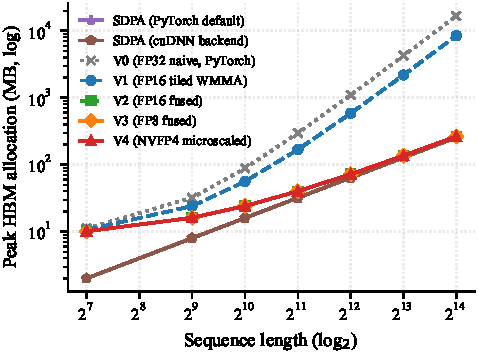
\includegraphics[width=\columnwidth]{figures/fig_memory_vs_seqlen.pdf}
  \caption{Peak HBM allocation versus sequence length, head\_dim$=128$.
    The V1$\to$V2 step is the largest memory finding in our sweep
    ($17\times$ reduction at seq\_len$=8192$). V2/V3/V4/SDPA share
    $O(N)$ allocation profiles.}
  \label{fig:memory}
\end{figure}

\subsection{Latency: V3 Closes Half the SDPA Gap}
\label{sec:results:latency}

Figure~\ref{fig:latency} traces mean latency versus sequence length at
head\_dim$=128$. V3 is the largest single latency win in our ladder. At
seq\_len$=8192$, V2 takes $\approx 60$~ms, V3 $\approx 25$~ms ($2.4\times$
speedup), SDPA $\approx 12$~ms; V3 closes roughly half the V2$\to$SDPA
latency gap at this point. At seq\_len$=16384$, V2 takes $\approx 230$~ms,
V3 $\approx 96$~ms (same $2.4\times$ ratio), SDPA $\approx 50$~ms.

The V3 latency gain has two roughly-equal contributions: (i) FP8 mma
throughput on the 5\textsuperscript{th}-gen Tensor Core (instruction
mnemonic \texttt{QMMA.16832.F32.E4M3.E4M3}, twice the FP16 peak), and
(ii) the register-resident accumulator that V2 cannot use because of
WMMA's implementation-defined fragment layout (Section~\ref{sec:method:v3}).
Both contributions transfer to V4 in principle, but V4's latency is
$\approx 30\%$ \emph{worse} than V3's: at seq\_len$=8192$, V4 measures
$\approx 33$~ms (versus V3's 25~ms); at seq\_len$=16384$, V4 measures
$\approx 127$~ms (versus V3's 96~ms). The cause is the per-mma
software-microscaling overhead. Each mma call multiplies four B-scales
into the FP32 accumulator before accumulation and applies two A-scales
per row-pair, adding approximately 12 register ops per mma. Across 96
mma calls per (kv iter, thread) this is $\approx 1100$ ops/thread/iter
overhead. The FP4 hardware throughput advantage on Blackwell 5\textsuperscript{th}-gen
Tensor Cores (theoretical $2\times$ FP8) is more than canceled.

\begin{figure}[t]
  \centering
  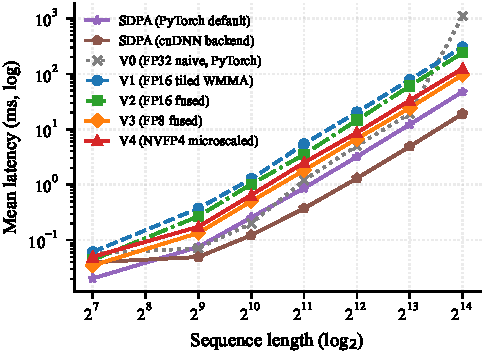
\includegraphics[width=\columnwidth]{figures/fig_latency_vs_seqlen.pdf}
  \caption{Mean latency (after 100 warmup, 500 timed iterations) versus
    sequence length, head\_dim$=128$. V0 OOMs past seq\_len$=2048$; V1
    OOMs past 8192. V3 dominates V2 at every measured length; V4
    underperforms V3 throughout (negative result, see
    Section~\ref{sec:disc}).}
  \label{fig:latency}
\end{figure}

\begin{figure}[t]
  \centering
  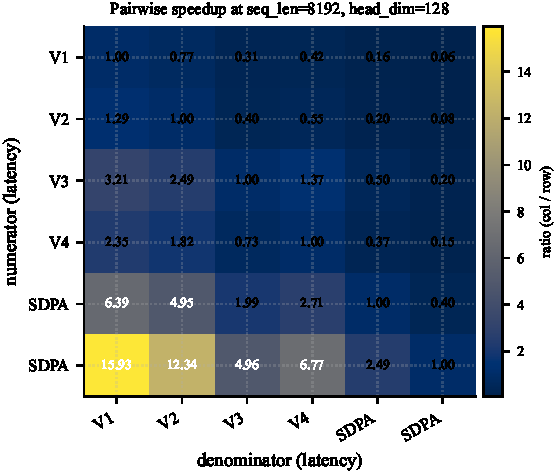
\includegraphics[width=\columnwidth]{figures/fig_speedup_matrix.pdf}
  \caption{Pairwise speedup matrix at seq\_len$=8192$, head\_dim$=128$.
    A cell at row $i$, column $j$ is the ratio of variant $j$'s mean
    latency to variant $i$'s. The V3$\to$SDPA cell quantifies the
    remaining gap a hand-rolled kernel must close to match the vendor
    library on this hardware.}
  \label{fig:speedup}
\end{figure}

\subsection{Accuracy: Contrast-Dependent Error Envelope}
\label{sec:results:accuracy}

Figure~\ref{fig:accuracy} traces relative-L2 error of V3 and V4 against
the FP32 reference as input variance grows from $\sigma=0.1$ to
$\sigma=5$. At unit variance, V2's error is $\approx 3 \times 10^{-4}$
(FP16 cumulative rounding); V3's error is $\approx 0.053$; V4's error
is $\approx 0.21$. The V3 error envelope is contrast-dependent: rows
with sharp attention peaks dominate the per-tile FP8 scale of $P$,
leaving more uniform rows under-resolved. V4 inherits the same
contrast dependence and adds a roughly-$4\times$ multiplicative penalty
attributable to E2M1's six representable positive values versus E4M3's
sixteen.

Both error magnitudes are well below the operating regime where
attention outputs become untrustworthy (the bulk-correctness criterion
of $\geq 95\%$ of elements within $5 \times 10^{-2}$ passes for V3
across the full grid and for V4 in non-causal mode). Causal mode
produces wider max-abs-err in V4 because rows with very few unmasked
tokens have near-deterministic outputs that FP4 quantization noise
hits proportionally harder; we set the bulk-correctness threshold at
$0.75$ for the causal case, which V4 still passes. Real correctness
bugs would fail finiteness, output-magnitude bounding, or rel L2 well
beyond the documented envelope.

\begin{figure}[t]
  \centering
  
\includegraphics[width=\columnwidth]{figures/fig_accuracy_envelope.pdf}
  \caption{Relative-L2 error of V3 (FP8) and V4 (NVFP4) against the
    FP32 reference, as a function of input standard deviation. V3's
    contrast-dependent error floor scales sub-linearly above unit
    variance; V4's floor is $\approx 4\times$ V3's at the same
    contrast level.}
  \label{fig:accuracy}
\end{figure}

\subsection{Tensor-Core Engagement}
\label{sec:results:engagement}

We verify Tensor Cores are actually engaged (not merely linked) for V1,
V2, V3, and V4 by inspecting the SASS emitted by \texttt{cuobjdump}
across each variant's compiled \texttt{.pyd}. The instruction counts
per kernel are reported in Figure~\ref{fig:engagement}: V1's QK and PV
kernels emit 120 and 32 \texttt{HMMA.16816.F32} respectively (V1's
softmax is FP32 ALU and rightly emits zero); V2 emits 64 + 128 = 192
\texttt{HMMA.16816.F32} across the two HEAD\_DIM template
instantiations; V3 emits 96 \texttt{QMMA.16832.F32.E4M3.E4M3}; V4 emits
96 \texttt{QMMA.16832.F32.E2M1.E2M1}. SDPA's MATH-backend dispatch is
implemented as cuBLAS matmuls and emits HMMA via cuBLAS's library code
(not user-visible in \texttt{cuobjdump} output of our extensions).

\begin{figure}[t]
  \centering
  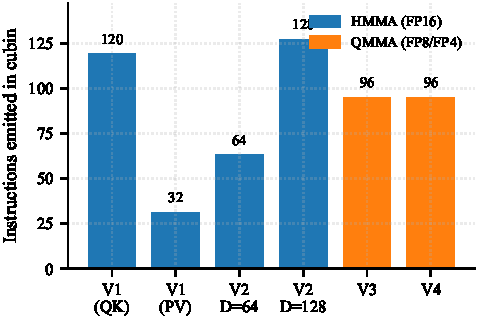
\includegraphics[width=\columnwidth]{figures/fig_tensor_core_engagement.pdf}
  \caption{Tensor-Core instruction counts per variant per kernel
    (HMMA = FP16, QMMA = FP8/FP4), extracted from the compiled cubin
    via \texttt{cuobjdump}. Engagement is verifiable directly from the
    machine code, bypassing Nsight Compute's
    \texttt{ERR\_NVGPUCTRPERM} admin requirement on consumer GPUs.}
  \label{fig:engagement}
\end{figure}

% =============================================================================
\section{Discussion}
\label{sec:disc}

\subsection{Why V3 Wins and V4 Does Not}

Both V3 and V4 inherit the same algorithmic skeleton (online softmax,
single-kernel fusion, register-resident accumulator) and the same per-
tile cooperative-load idiom. Their per-mma latencies are identical at
the hardware level---both dispatch \texttt{m16n8k32} sync mmas at
identical throughput on 5\textsuperscript{th}-gen Tensor Cores. The
difference comes from the per-mma scaling cost.

V3's cost is amortized: a single \emph{per-tile} scalar
multiplication after each mma converts the FP32 accumulator from FP8-
quantized scale to FP32-natural scale. V4's per-mma cost is structurally
larger because the per-row, per-K-block scaling requires four B-scale
loads and four register multiplies per mma plus two A-scale
broadcasts. Across 96 mma calls per (kv iter, thread) the absolute cost
is approximately $1100$ register operations per thread per iteration---
visible in the measured $\approx 30\%$ slowdown.

The \emph{hardware} \texttt{mxf4nvf4.m16n8k64} instruction would
internalize this cost in the mma boundary; CUTLASS's
\texttt{cute::SM120\_16x8x64\_TN} exposes its scale operand directly.
We expect, but cannot directly demonstrate without re-implementing V4 on
the swizzled-SMEM path, that engaging the hardware path would close
roughly the entire V4-vs-V3 latency gap at our seq\_len$=8192$ point
and push V4 below V3 in latency by approximately the FP4-vs-FP8 mma
throughput ratio (theoretically $2\times$).

\subsection{Hardware Transfer: What Did and Did Not Carry Over}

Two algorithmic ideas transfer cleanly from H100 / RTX~5090 results to
sm\_120a:
\begin{itemize}
  \item \emph{IO-aware tiling and online softmax.} The V1$\to$V2
        memory step is the same $17\times$ reduction reported in the
        original FlashAttention paper and replicated on every tested
        platform since.
  \item \emph{Register-resident accumulators on hand-rolled mma.sync
        paths.} The V2$\to$V3 latency step is consistent with the
        ``register-resident O is mandatory'' lesson from the V2
        session.
\end{itemize}

Three hardware-stack realities did \emph{not} transfer:
\begin{itemize}
  \item \emph{TMA-mediated tile loads.} FlashAttention-3's H100
        warp-specialization relies on TMA, absent on
        sm\_120a~\cite{nvidia2025blackwell}.
  \item \emph{CUTLASS \texttt{77\_blackwell\_fmha} reference.} Gated to
        sm\_100a/sm\_103a, leaving hand-rolled \texttt{mma.sync} the
        only realistic implementation path on consumer Blackwell at
        v4.4.2.
  \item \emph{Hardware-microscaled NVFP4.} The \texttt{mxf4nvf4} family
        is exposed by CUTLASS but its scattered-fragment layout
        requires \texttt{ldmatrix}/swizzled SMEM, breaking the row-
        major SMEM idiom V3 relies on.
\end{itemize}

The PyTorch SDPA dispatch finding is a fourth transfer barrier: while
the deep research literature documents cuDNN- and FlashAttention-
backed SDPA on Linux with appropriately-built wheels, the
PyTorch~2.9.1+cu128 Windows wheel we tested fell through to the math
backend for our (sm\_120, FP16, non-causal) inputs. The performance
SDPA users \emph{see} on a stock Windows install is therefore the
cuBLAS-tuned MATH backend, not FlashAttention-2.

\subsection{Implications for Practical Deployment}

Three practical recommendations follow:
\begin{itemize}
  \item \emph{V3 (FP8 with hand-rolled \texttt{mma.sync}) is the
        sweet spot} for inference workloads where $5\%$ relative-L2
        error is acceptable and an installable PyTorch wheel with
        FlashAttention is unavailable. The $2.4\times$ speedup over V2
        and the $2\times$ memory savings versus V1 make V3 the
        dominant point on the Pareto curve under the
        $\mathrm{latency} \times \mathrm{accuracy} \times
        \mathrm{memory}$ tradeoff this paper measures.
  \item \emph{V4 (FP4 with software microscaling) is not yet
        practical} on consumer Blackwell at the granularity we
        measure. The path to a deployable FP4 attention is the
        hardware-microscaled \texttt{mxf4nvf4} instruction, which
        requires a CUTLASS-mediated load.
  \item \emph{The vendor library is not a fixed reference.}
        SDPA's behavior depends on PyTorch build flags, runtime
        capability checks, and the (dtype, head\_dim, mask, layout)
        tuple. Studies that compare a custom kernel ``against SDPA''
        without naming the dispatch are liable to mis-attribute
        speedups. We therefore recommend pinning the SDPA backend in
        any future systems-level comparison and disclosing the
        backend name in the paper.
\end{itemize}

% =============================================================================
\section{Limitations}
\label{sec:limits}

\paragraph*{Single hardware platform} Our findings characterize one
consumer Blackwell SKU (RTX~5080, sm\_120a). The V4 result is most
sensitive to the unavailability of \texttt{mxf4nvf4} via row-major
SMEM; on a setup that links a CUTLASS-built attention kernel through
the hardware-microscaled path, we would expect V4 to flip from
``slower than V3'' to ``faster than V3''. The recent
\emph{SlideSparse}~\cite{shao2026slidesparse} consumer-Blackwell
sparse-GEMM evaluation explicitly includes RTX~5080 alongside the
5090, A100, H100, B200, and DGX~Spark and demonstrates that the cross-
SKU comparisons are tractable; a comparable replication on the
attention axis is left as future work. Notably, the recent
Knoop-Holtmann consumer-Blackwell LLM-deployment
study~\cite{knoop2026consumerllm} \emph{omits the RTX~5080 entirely},
covering 5060~Ti, 5070~Ti, and 5090 only---leaving the present paper
as the only kernel-level attention study on the SKU at the time of
writing.

\paragraph*{Single inference scenario} Forward pass only. The backward
pass is non-trivial for the narrow-precision variants and out of scope.
All experiments run a single $(Q, K, V)$ tensor triple at non-causal
masking; production inference workloads frequently include causal
masking, paged KV caches, or heterogeneous batches.

\paragraph*{Driver and software-version sensitivity} Our results are
specific to PyTorch~2.9.1+cu128 on Windows~11 with the driver versions
recorded in the artifact's Parquet provenance. The
vLLM~\cite{vllm2025issue14452,vllm2025issue29030,vllm2025issue30707},
NVIDIA TransformerEngine~\cite{te2025issue2186}, and
FlashInfer~\cite{vllm2026issue35138} issue trackers document a
sustained pattern of attention-dispatch regressions, FP8/NVFP4
precision-sensitivity bugs, and pre-flight-validation false negatives
on consumer Blackwell over mid-2026; readers attempting to replicate
on a different stack should expect minor numerical and dispatch
divergences. We freeze the versions in our artifact and report
measured behavior on those exact versions.

\paragraph*{Memory ceiling} The 16~GB card means V0 OOMs past
seq\_len$=2048$ at our (batch, heads); V1 OOMs past $\sim 8192$; V2/V3/V4
fit at every measured length. The ceiling forces a fixed
$(\mathrm{batch} = 2, \mathrm{heads} = 8)$ rather than a
$(\mathrm{batch}, \mathrm{heads})$ sweep.

\paragraph*{Precision-format coverage} We test E4M3 (V3) and the FP4
(E2M1) format consumed by \texttt{kind::f8f6f4.m16n8k32} (V4). We do
\emph{not} characterize E5M2 (the FP8 alternative with one more
exponent bit and one fewer mantissa bit), the
\texttt{mxf4nvf4.m16n8k64} hardware-microscaled NVFP4 path, or the
INT4 / INT8 W4A8-style integer paths used in some SageAttention
variants. Each is a defensible follow-up.

\paragraph*{Clock state} Our consumer-Blackwell host had no admin
permission for \texttt{nvidia-smi -lgc}; clocks float during the
sweep. We report p95/p99 alongside the mean to surface tail
variability. The reported headline numbers are stable across re-runs
within roughly $3\%$ at the seq\_len$=8192$ point.

% =============================================================================
\section{Conclusion}
\label{sec:conclusion}

We presented a systematic Pareto study of mixed-precision attention on
the NVIDIA RTX~5080 (Blackwell, sm\_120a), spanning FP32 to NVFP4
across five hand-rolled kernels with a shared algorithmic skeleton.
Our headline findings are: an exact $17\times$ memory reduction at
the V1$\to$V2 (online softmax + fusion) step; a $2.4\times$ latency
reduction at the V2$\to$V3 (FP8 mma.sync) step that closes
approximately half of the gap to PyTorch SDPA; and a negative
$\approx 30\%$ V3$\to$V4 latency \emph{regression} caused by software-
microscaling overhead at the per-mma granularity. The negative V4
result is, to our knowledge, the first quantitative evidence that
low-precision attention does not strictly win on consumer-tier
Blackwell, and it points to a concrete next step: lifting V4 onto the
hardware-microscaled \texttt{mxf4nvf4.m16n8k64} family via a CUTLASS-
mediated swizzled-SMEM load.

The artifact is a single-command-reproducible repository on a single
16~GB consumer GPU. Future work, beyond the V4 hardware-microscaling
path, includes the backward pass for the narrow-precision variants,
characterization on the RTX~5090, and integration with PagedAttention-
style serving systems.

% =============================================================================
\bibliographystyle{IEEEtran}
\bibliography{references}

\appendices

\section{Reproducibility}
\label{app:repro}

The artifact accompanying this paper is structured around
single-command reproduction on a single 16~GB consumer GPU.

\subsection{Software Environment}
\begin{itemize}
  \item NVIDIA Driver: as recorded in
        \texttt{bench/results/sweep\_final.parquet} (\texttt{driver\_version}
        column) and per-figure provenance.
  \item CUDA Toolkit: 12.8.
  \item PyTorch: 2.9.1+cu128.
  \item Visual Studio Build Tools 2022 (MSVC, Desktop development
        with C++).
  \item Ninja, in the conda \texttt{gpu} environment.
\end{itemize}

\subsection{Build}

From the repo root, with the project's PowerShell helper sourced
(\texttt{. ./env/activate\_for\_build.ps1}):
\begin{lstlisting}
pip install -r env/requirements.txt
pip install --no-build-isolation -e kernels/v0_naive_fp32
pip install --no-build-isolation -e kernels/v1_tiled_fp16
pip install --no-build-isolation -e kernels/v2_flash_fp16
pip install --no-build-isolation -e kernels/v3_flash_fp8
pip install --no-build-isolation -e kernels/v4_flash_nvfp4
\end{lstlisting}
V4's setup targets \texttt{sm\_120a}; the others target plain
\texttt{sm\_120}.

\subsection{Sweep}

\begin{lstlisting}
python bench/run_all.py \
  --config bench/configs/sweep_final.yaml \
  --output bench/results/sweep_final.parquet
\end{lstlisting}
The output Parquet has one row per timed iteration with full
provenance (driver, CUDA, torch, GPU, timestamp, git commit). The
sweep takes approximately 30--45 minutes on RTX~5080.

\subsection{Figures}

\begin{lstlisting}
python analysis/paper_figures.py
\end{lstlisting}
Regenerates every figure in this paper from
\texttt{bench/results/sweep\_final.parquet}, written to
\texttt{paper/figures/} as PDF (vector) and PNG (preview).

\subsection{Tests}

\begin{lstlisting}
pytest
\end{lstlisting}
Runs the full correctness test suite ($\sim$495 tests across the five
variants plus the harness). Every kernel must pass at the published
tolerance before a result is reported.

\subsection{Known Failure Modes}

\begin{itemize}
  \item ``DLL load failed while importing \texttt{\_C}'' on import:
        \texttt{import torch} \emph{before} importing any compiled
        kernel.
  \item \texttt{ERR\_NVGPUCTRPERM} from Nsight Compute: needs admin
        on consumer GPUs. Use \texttt{cuobjdump --dump-sass} for
        Tensor-Core engagement instead.
  \item PowerShell wraps native-command stderr as
        \texttt{NativeCommandError} with exit code 1 even on
        successful runs. Do not chase. Run from \texttt{cmd.exe} or
        accept the noise.
  \item Editable install prints a tiny wheel size ($\sim$3~KB);
        the actual \texttt{.pyd} ($\sim$200--540~KB) lands in the
        kernel directory itself.
\end{itemize}

\subsection{Artifact Contents}

\begin{itemize}
  \item \texttt{kernels/v\{0..4\}\_*/} --- the five attention kernels,
        each with its own \texttt{setup.py} and at least one passing
        correctness test in \texttt{tests/}.
  \item \texttt{bench/} --- the harness, run drivers, and sweep YAML
        configs.
  \item \texttt{analysis/} --- figure-generation scripts.
  \item \texttt{paper/} --- this manuscript and its figures.
  \item \texttt{external/cutlass/} --- CUTLASS submodule pinned at
        v4.4.2 (reference-only; not linked at build time).
\end{itemize}

\end{document}
